\section{Menedżery pakietów w systemie Linux}

Lorem ipsum..

\subsection{Flatpak}



Flatpak \cite{flatpak-future} to jeden z najpopularniejszych uniwersalnych menedżerów pakietów.

 co zostało zilustrowane na rysunku \ref{fig:flatpak-schemat}.

\begin{figure}[htbp]
    \centering
    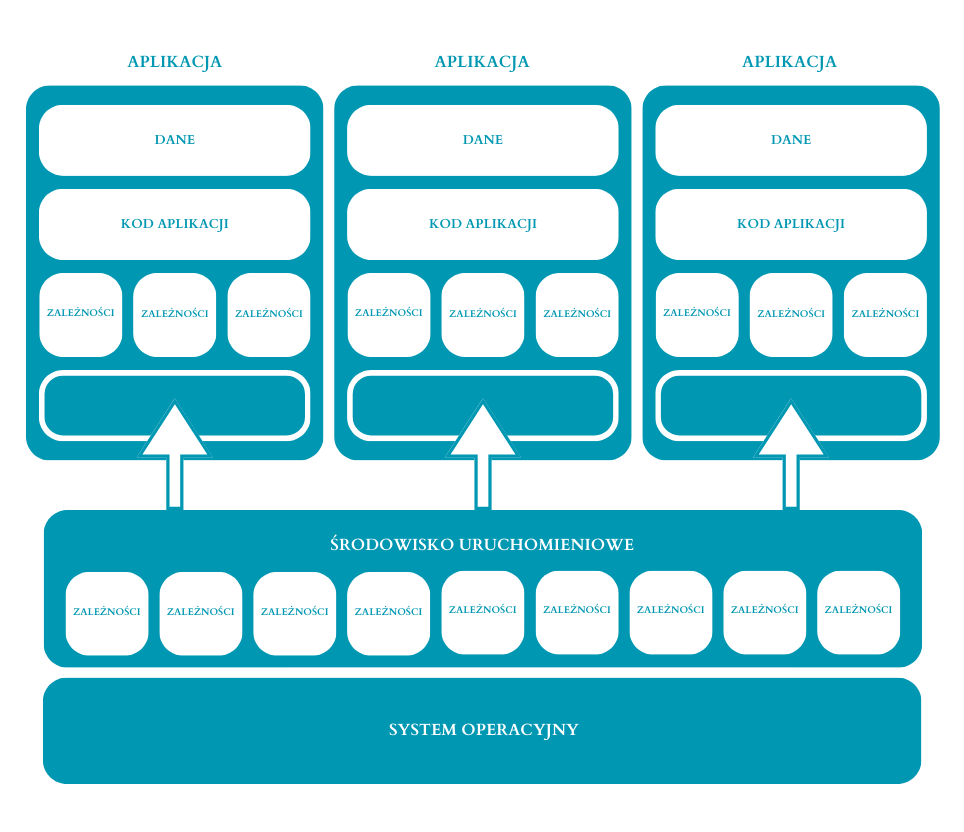
\includegraphics[width=\linewidth]{img/schematy/flatpak_schemat.png}
    \caption{Schemat ilustrujący działanie izolacji w menedżerze pakietów Flatpak}
    \label{fig:flatpak-schemat}
\end{figure}

Lorem

\subsection{Snap}

Lorem

\subsection{AppImage}

Lorem